\documentclass[oupdraft]{bio}
%\usepackage[colorlinks=true, urlcolor=citecolor, linkcolor=citecolor, citecolor=citecolor]{hyperref}
\usepackage{natbib}
\usepackage{amsmath,amssymb}
\usepackage[plain,noend]{algorithm2e}
\usepackage{xspace}
% Add history information for the article if required
% \history{Received August 1, 2010;
% revised October 1, 2010;
% accepted for publication November 1, 2010}

\def\aic{\textsc{aic}\xspace}
\def\bic{\textsc{bic}\xspace}
\def\ric{\textsc{ric}\xspace}
\def\forward{\textsc{forward}\xspace}
\def\last{\textsc{last}\xspace}
\def\T{{ \mathrm{\scriptscriptstyle T} }}
\def\v{{\varepsilon}}
\def\real{{\mathbb R}}
\def\pen{{\mathcal P}}
\DeclareMathOperator*{\argmax}{arg\,max}
\DeclareMathOperator*{\argmin}{arg\,min}
\newcommand{\norm}[1]{\lVert #1 \rVert}
\newcommand{\vecsp}{\mathcal{L}}
\newcommand{\maximize}{\mathop{\mathrm{maximize}}}

\newenvironment{definition}[1][Definition]{\begin{trivlist}
\item[\hskip \labelsep {\bfseries #1}]}{\end{trivlist}}

\SetAlCapSkip{1em}

\begin{document}

% Title of paper
\title{A significance test for forward stepwise model selection}

% List of authors, with corresponding author marked by asterisk
\author{JOSHUA R. LOFTUS$^\ast$, JONATHAN E. TAYLOR\\[4pt]
% Author addresses
\textit{Department of Statistics,
Stanford University,
290 Serra Mall, Stanford, CA,
United States}
\\[2pt]
% E-mail address for correspondence
{joftius@stanford.edu}}

% Running headers of paper:
\markboth%
% First field is the short list of authors
{J. R. Loftus and J. E. Taylor}
% Second field is the short title of the paper
{Forward stepwise significance test}

\maketitle

% Add a footnote for the corresponding author if one has been
% identified in the author list
\footnotetext{To whom correspondence should be addressed.}

\begin{abstract}
{We propose a new significance test for variables
chosen in forward stepwise model selection.
The test statistic has an
exact truncated chi distribution at the first step conditional on the
variable chosen. Iterating the test on the residual after each step
yields a sequence of conditional $p$-values which we interpret as
tests for the inclusion of each variable conditional on the model
chosen up to that point. Simulations show the test is powerful and
becomes increasingly conservative after forward stepwise has added all
the truly nonzero variables. The resulting method has the
computational strengths of stepwise selection and addresses the
problem of invalid test statistics due to model selection.}
{Forward stepwise; Model selection; Significance test}
\end{abstract}


\section{Introduction}

Forward stepwise regression is a regression model selection procedure
that begins with an empty model and sequentially adds the best
predictor variable in each step. Since forward stepwise uses the data
to choose variables, the usual $\chi^2$ and $F$-tests for significance
are invalid when a model has been selected this way
\citep{olshen:flevel}.
These tests will
be anti-conservative unless they are computed on a held-out validation
dataset. This is an instance of the general problem of conducting
inference and model selection using the same data. In the lasso setting,
\cite{significance:lasso} derived a novel test
statistic with an asymptotic exponential distribution under the null.
\cite{tests:adaptive} modified and extended those
results to the group lasso \citep{bakin:grouplasso,grouplasso} and other penalized regression problems, but only under the global null.
The present work iteratively applies the global null test of
\cite{tests:adaptive} on the residual in each step in forward stepwise
and works out the details necessary for models with grouped
variables.
These tests can be used for
valid significance testing when computed on the same data used for
model selection, eliminating the need for data splitting. This is
important when data splitting is not appropriate, for
example, when categorical covariates have levels with very few
observations.

Forward stepwise adds the ``best'' variable into the model, and our test is
based roughly on comparing the improvement gained from adding this variable
to the improvement possible using the {\em second best} variable.
For intuition, consider the simple case when $y_i \sim N(\mu_i,1)$
for $i = 1,\ldots,n$
are independent and the design matrix $X = I$. Forward stepwise chooses the
largest $|y_i|$ to add to the model. Under the null, this value will be
on the order of $\sqrt{2 \log (n)}$. This is highly significant for a
$N(0,1)$ random variable, so the $\chi^2$ test will fail.
However, the second largest $|y_i|$ will be only slightly smaller, and our
test uses this information to form a valid test for the largest. Under a
sparse alternative in order for any test to have power the nonzero
$\mu_i$ must be larger than $\sqrt{2 \log (n)}$. In this case, 
the gap in improvement between the last truly nonzero $\mu_i$ added by
forward stepwise and the remaining noise variables should be large,
hence detectible by our test.

In the general setting without $X = I$, our statistic can be understood 
as the survival function of the random variable
\begin{equation}
\label{eq:lam1}
\lambda_1 = \|X^Ty\|_{\infty}
\end{equation}
{\em conditional} on which variable achieves the maximum and its sign.
Under the null, and ignoring the maximum for a moment, this quantity is
a $\chi$ random variable with some degrees of freedom $r$ and scale
$\theta$ depending on $X$. Accounting for the maximum by conditioning requires
a truncation set $M \subset \real^+$ given by the fact that we observe
$\lambda_1 \geq m$, where $m$ is determined by the ``second best'' variable.
With these ingredients and the relevant survival function we now define
our test.
\begin{definition}
The {\em truncated $\chi$ test statistic} is
\begin{equation}
\label{eq:tchi}
T\chi(\lambda_1, r, \theta,  M) = \frac{\int_{M /\theta \cap [\lambda_1/\theta,\infty)} F_{\chi_r}(dz)}{\int_{M / \theta} F_{\chi_r}(dz)}
\end{equation}
with explicit formulas for $r$, $\theta$, and $M$ given in
Algorithms~\ref{algo:pval}--\ref{algo:linfrac}.
\end{definition}

The main result in \cite{tests:adaptive} shows that
$T\chi \sim \text{Unif}([0,1])$ under the global null. In forward stepwise
we iterate this test on the residual after each step, and show in simulations
that it performs well.

\section{Forward stepwise model selection}
%%%%%%%%%%%%%%%%%%%%%%%%%%%%%%%%%%%%%%%%%%%%%%%%%%%%%%%%%%%%%%%%%%%%%%%

\subsection{Background and notation}

Forward stepwise regression is a classical method, reviewed in
\cite{classical:selection}, which continues to be widely used by
practitioners despite the fact that it invalidates inferences using
the standard $\chi^2$ or $F$-tests. Some attempts to address this
issue include Monte Carlo estimation of tables of adjusted
$F$-statistic values \citep{mc:ftoenter} and permutation tests
\citep{permutation:stop}. Aside from the works this paper is based on,
there have been other recent attempts to do inference after model
selection. Most of these make use of subsampling
\citep{meinshausen:buhlmann} or data splitting
\citep{wasserman:roeder}. Our approach allows use of the full data and
does not require the extra computation involved in subsampling.

Our variant of forward stepwise is described in Algorithm~\ref{algo:fs}.
We allow arbitrary predefined groups of variables, so our method can be
used with categorical variables or factor models.
To emphasize this we use $g, h$ as covariate indices rather than
the usual $i, j$ throughout. Since single variables can be considered
groups of size 1, this includes non-grouped situations as a special
case. Let $y \in \real^n$ be $n$ measurements of the outcome
variable, not necessarily independent.
Let an integer $G \geq 2$ be the number of groups of
explanatory variables. For each $1 \leq g \leq G$ the design matrix
encoding the $g$th group is the $n \times p_g$ matrix denoted $X_g$,
where $p_g$ is the number of individual variables or columns in group
$g$. With categorical variables by default we use the full encoding with
one column for every level.
Denote by $p = \sum_{g=1}^Gp_g$ the total number of individual
variables, so $p = G$ in the case where all groups have size 1. Let
$X$ be the matrix constructed by column-binding the $X_g$, that is
%%%%%%%%%%%%%%%%%%%%%%%%%%%%%%%%%%%%%%%%%%%%%%%%
\begin{equation*}
X = \begin{pmatrix} X_1 & X_2 & \cdots & X_G  \end{pmatrix}
\end{equation*}
%%%%%%%%%%%%%%%%%%%%%%%%%%%%%%%%%%%%%%%%%%%%%%%%
We also allow weights $w_g$ for each group. These
weights act like penalties or costs, so increasing $w_g$ makes it
more difficult for the group $X_g$ to enter the model. The
modeler can choose weights arbitrarily for calibration purposes,
for example to account for groups having different sizes.
Throughout we set all weights to 1 and normalize
groups by the Frobenius norm of their corresponding submatrices.

With each group we associate the $p_g \times 1$ coefficient vector
$\beta_g$, and write $\beta$ for the $p \times 1$ vector constructed
by stacking all of the $\beta_g$ in order.  Finally, our model for the
response is
\begin{equation}
\label{eq:gmodel}
y  = X \beta + \sigma \epsilon  = \sum_{g=1}^G X_g \beta_g + \sigma \epsilon
\end{equation}
where $\epsilon$ is noise. We assume Gaussian noise
$\epsilon | X \sim N(0, \Sigma)$ with known covariance matrix $\Sigma$.
The model \eqref{eq:gmodel} is underdetermined when $p > n$.
In such cases it still may be possible to
estimate $\beta$ well if it is sparse, that is it has few nonzero
entries. In the rest of this paper we refer to variable groups $X_g$
as noise groups if $\beta_g$ is a zero vector and as true or signal
groups if $\beta_g$ has any nonzero entries. We refer to the number
of such nonzero groups as the sparsity of the model, and
denote this $k := \# \{ g : \beta_g \neq 0 \}$.

Before using Algorithm~\ref{algo:fs}
the user must specify the maximum number of steps allowed,
which we denote \textit{steps}.
To enable $T\chi$ statistic computations,
\textit{steps} should be at most $\min (n, G) - 1$. It is
computationally desirable to set it as low as possible while
remaining safely larger than the sparsity of $\beta$
so that forward stepwise may recover all the nonzero
coefficients of $\beta$ and terminate without performing much
additional computation. Since the sparsity is usually unknown this
requires some guesswork.

\begin{figure}
\begin{algorithm}[H]
  \caption{Forward stepwise variant with groups and weights}
  \label{algo:fs}
    \SetAlgoLined
    \DontPrintSemicolon
    \KwData{An $n$ vector $y$ and $n \times p$ matrix $X$ of $G$ variable groups with weights $w_g$}
    \KwResult{Ordered active set $A$ of variable groups included in the model at each step}
    \Begin{
    $A \leftarrow \emptyset$, $A^c \leftarrow \{ 1, \ldots, G\}$, $r_0 \leftarrow y$\;
    \For{$s=1$ \KwTo $steps$}{
        $g^* \leftarrow \argmax_{g \in A^c} \{ \lVert X_g^Tr_{s-1} \rVert_2 / w_g \}$\;
        $P_{g^*} \leftarrow I_{n\times n} - X_{g^*}X_{g^*}^\dagger$\;
        $A \leftarrow A \cup \{ g^* \}$, $A^c \leftarrow A^c \backslash \{ g^* \}$\;
        \For{$h \in A^c$}{
            $X_h \leftarrow P_{g^*} X_h$\;
        }
        $r_s \leftarrow P_{g^*} r_{s-1}$\;
    }
    \KwRet{$A$}
    }
\end{algorithm}
\end{figure}

The active set $A$ contains variable groups chosen to be included in
the model. Fitting $\hat \beta$ can be done by tracking the individual
fits and projections, or by refitting a linear model on the submatrix
of $X$ corresponding to $A$. Other implementations of forward stepwise
use different criteria for choosing the next variable to add, such as
the correlation with the residual. Since we do not renormalize the
columns after projecting the covariates, and
since we have weights, we are not generally computing correlations
unless the design matrix is orthogonal and all weights are 1.
We use forward stepwise to refer specifically to
Algorithm~\ref{algo:fs}.


\section{Significance testing with model selection}
\label{sec:testing}
%%%%%%%%%%%%%%%%%%%%%%%%%%%%%%%%%%%%%%%%%%%%%%%%%%%%%%%%%%%%%%%%%%%%%%%

\subsection{Previous work}

To describe previous work we require some facts about the solution
path of the lasso summarized in
\cite{significance:lasso,tibshirani_lasso_uniqueness}.
Recall that the lasso estimator is 
%%%%%%%%%%%%%%%%%%%%%%%%%%%%%%%%%%%%%%%%%%%%%%%%
\begin{equation}
\begin{aligned}
\label{eq:lasso}
\displaystyle \hat \beta(\lambda) = \argmin_{\beta \in \real^p} \frac{1}{2} \| y - X \beta \|_2^2 +
   \lambda \| \beta \|_1. \\
\end{aligned}
\end{equation}
%%%%%%%%%%%%%%%%%%%%%%%%%%%%%%%%%%%%%%%%%%%%%%%%


\begin{itemize}
\item The vector valued function $\hat \beta(\lambda)$ is a continuous
function of $\lambda$. For the lasso path, the coordinates of $\hat
\beta(\lambda)$ are piecewise linear with changes in slope occurring
at a finite number of $\lambda$ values referred to as \emph{knots}.

\item The knots depend on the data and are usually written in order
$\lambda_1 \geq \lambda_2 \geq \cdots \geq \lambda_r \geq 0$.
\end{itemize}

\cite{significance:lasso} introduced the \emph{covariance test} which
is based on the lasso solution path knots. They derived a simple
asymptotic null distribution, proved a type of convergence under broad
``minimum growth'' conditions, and demonstrated in simulations that
the test statistic closely matches its asymptotic distribution even in
finite samples. Assuming $\Sigma = \sigma^2 I$, the covariance test is
given at the first step by
\begin{equation}
\label{eq:covtest}
T_1 = \frac{\lambda_1(\lambda_1-\lambda_2)}{\sigma^2} \overset{n,p \to \infty}{\to} \text{Exp}(1).
\end{equation}
This is a hypothesis test for including the first variable in the lasso
path, with large values of the test statistic being evidence against the
global null. 
The limiting results about later steps in \cite{significance:lasso} can be interpreted as recursively applying $T_1$ to the variables that had not previously been selected by lars.
\cite{tests:adaptive} observed
\begin{equation}
\label{test:exact}
\exp\left(- \frac{\lambda_1(\lambda_1-\lambda_2)}{\sigma^2} \right)
\approx
\frac{1 - \Phi(\lambda_1/\sigma)}{1 - \Phi(\lambda_2 / \sigma)} \overset{D}{=} \text{Unif}([0,1])
\end{equation}
with the exact, finite sample distribution on the right hand side holding
under the global null.
Further, their test is also general enough to handle the group lasso and other penalized regression methods. The group lasso estimator \citep{bakin:grouplasso,grouplasso}, a generalization of the lasso, is a solution to the following penalized least-squares convex problem
%%%%%%%%%%%%%%%%%%%%%%%%%%%%%%%%%%%%%%%%%%%%%%%%
\begin{equation}
\begin{aligned}
\label{eq:gsoln}
\displaystyle \hat \beta_\lambda = \argmin_{\beta \in \real^p} \frac{1}{2} \| y - X \beta \|_2^2 +
   \lambda {\cal P}(\beta) \\
\end{aligned}
\end{equation}
%%%%%%%%%%%%%%%%%%%%%%%%%%%%%%%%%%%%%%%%%%%%%%%%
with the group penalty
%%%%%%%%%%%%%%%%%%%%%%%%%%%%%%%%%%%%%%%%%%%%%%%%
\begin{equation}
  \begin{aligned}
  \label{eq:gpen}
    {\cal P}(\beta)&= \sum_{g=1}^G w_g \| \beta_g \|_2 \\
  \end{aligned}
\end{equation}
%%%%%%%%%%%%%%%%%%%%%%%%%%%%%%%%%%%%%%%%%%%%%%%%
The parameter $\lambda \geq 0$ enforces sparsity in groups: for large
$\lambda$ most of the $\beta_g$ will be zero vectors. The weights
$w_g$ are usually taken to be $\sqrt {p_g}$ to normalize the penalty
across groups with different sizes.
This includes the usual lasso estimator as a
special case when all groups are of size 1, since then the
penalty term is the $\ell_1$-norm of $\beta$. The solution path of the group
lasso has similar properties to the lasso case, however it is not
generally piecewise linear.

The relation of lasso and group lasso to the present test is that
$T\chi$ is based on $\lambda_1$. Recall that
for sufficiently large $\lambda$ the solution to~\eqref{eq:gsoln} is forced
to be zero. The smallest such $\lambda$ is denoted
%%%%%%%%%%%%%%%%%%%%%%%%%%%%%%%%%%%%%%%%%%%%%%%%
\begin{equation}
  \begin{aligned}
   \lambda_1 &= \inf \{ \lambda \geq 0 : \hat \beta_{\lambda'} = 0 \text{ for all } \lambda' > \lambda \} \\
  \end{aligned}
\end{equation}
%%%%%%%%%%%%%%%%%%%%%%%%%%%%%%%%%%%%%%%%%%%%%%%%
For the group lasso this is explicitly computable by
\begin{equation}
%\label{eq:lammax}
\lambda_1^{\text{group}} = \max_{g} \frac{1}{w_g}\|X_g^Ty\|_2
 = \frac{1}{w_{g^*}}\eta_{g^*}^TX_{g^*}^Ty .
\end{equation}
where $g^*$ is the group that achieves the maximum and
$\eta_{g^*} = X_{g^*}^Ty / \|X_{g^*}^Ty\|_2$ is the unit vector that
achieves the norm $\|X_{g^*}^Ty\|_2$. 
The $T\chi$ test conditions on both the maximizer $g^*$ and
on the unit vector $\eta_{g^*}$.

\subsection{The $T\chi$ test statistic}

For the rest of this section let $g = g^*$ be the index of the group attaining the maximum in Algorithm~\ref{algo:fs}. Computing the $T\chi$ statistic when this group has size larger than 1 requires a bit of extra work. For groups of size one, the sign $\eta_g = \pm 1$, but for larger groups $\eta_g$ is a unit vector, and this is roughly why we need to form the projection matrix in \eqref{eq:proj}.

The underlying Gaussian process theory in \cite{tests:adaptive} studies the process $\eta \mapsto \eta^TX^Ty$ with $\eta$ in some parameter space. With nontrivial groups the parameter space is a manifold with nontrivial tangent spaces. In this case studying the maximum and maximizer necessitates forming an orthogonal projection to the tangent space $\vecsp_g = \{ u \in \real^p : u_g^T X_g^T y = 0, u_h = 0 \text{ for all } h \neq g \}$. If $X_g$ is a single column and $X_g^Ty \neq 0$, which should be the case since $g$ maximizes the norm of this quantity, then the space is trivial and the desired orthogonal projection is the identity. Otherwise, if $X_g$ has $p_g > 1$ columns the space $\vecsp_g$ generally has dimension $p_g-1$. We compute an orthonormal basis by Gram-Schmidt and form a $p_g \times p_g$ matrix, which we denote $V_g$, by appending an additional column of zeroes since Gram-Schmidt only produces $p_g-1$. We can now define the $n \times n$ projection
\begin{equation}
   \label{eq:proj}
   P_g = \Sigma X_gV_g (V_g^T X_g^T \Sigma X_g V_g)^\dagger V_g^TX_g^T. \\
\end{equation}
Also define $H_g = (I-P_g)\Sigma$, and the conditional variance
\begin{equation}
   \label{eq:cvar}
   \sigma^2_g = y^TX_gX_g^T H_g X_gX_g^Ty / (w_g^2 \norm{X_g^Ty}_2^2) \\
\end{equation}
which will ultimately be the scale $\theta$ of the truncated $\chi$.
These simplify when $X_g$ is a single column, in which case $P_g = 0$,
$H_g = \Sigma$, and $\sigma^2_g = X_g^T\Sigma X_g^T/w_g^2$.
Finally, with $F_{\chi^2_r}$ denoting the distribution function of a $\chi^2$ random variable with $r$ degrees of freedom, we are ready to describe the computation of $T\chi$ in Algorithm~\ref{algo:pval}.

\begin{figure}
\begin{algorithm}[H]
 \caption{Computing the $T\chi$ $p$-value} \label{algo:pval}
 \SetAlgoLined
 \DontPrintSemicolon
   \KwData{Residual $r$, grouped design matrix $X$ with weights, known covariance $\Sigma$, inactive set $A^c$, index $g$ of last group to enter active set $A$.}
   \KwResult{$T\chi$ $p$-value for the group $g$ entering the model.}\;
   \Begin{
   \eIf{$p_g = 1$}{
     $\sigma_g^2 \leftarrow X_g^T\Sigma X_g/w_g^2$\;
     $U_g \leftarrow X_g / w_g \cdot \text{sign}(X_g^Tr)$\;
   }{
     $H_g \leftarrow (I - P_g)\Sigma$ \tcp*{using $P_g$ from \eqref{eq:proj}}
     $\theta \leftarrow \sigma^2_g$ \tcp*{see \eqref{eq:cvar}}
     $U_g \leftarrow H_g X_g X_g^T r /(\norm{X_g^Tr}_2 w_g)$\;
   }
   $\lambda \leftarrow \norm{X_g^Tr}_2/w_g$\;
   $a \leftarrow X^T(y - \lambda U_g)$\;
   $b \leftarrow X^T U_g$\;
   $(v_-, v_+) \leftarrow \textsc{LinearFractional}(a,b)$
     \tcp*{Algorithm~\ref{algo:linfrac}}
   $r \leftarrow \text{rank}(X_g)$\;
   \KwRet{$[F_{\chi^2_r}(v^2_-/\theta) - F_{\chi^2_r}(\lambda^2/\theta)]/[F_{\chi^2_r}(v^2_-/\theta) - F_{\chi^2_r}(v^2_+/\theta)]$}
   }
\end{algorithm}
\end{figure}
The \textsc{LinearFractional} optimization subproblem referred to in
Algorithm~\ref{algo:pval} is, intuitively, finding the ``second best''
value that we use to evaluate the significance of $\lambda_1$. It returns
the truncation set $M = (v_-, v_+)$. 
Up to some constraints, the problem is finding the maximum and minimum of
\begin{equation}
\label{eqn:linfrac}
\frac{u_h^T a_h }{1 - u_h^T b_h} \qquad h \neq g, \norm{u_h}_2 = 1
\end{equation}
on two different sets.
The constraints, given by Lemma 1 in \cite{tests:adaptive}, incorporate the information that $g$ maximizes $\norm{X_g^Ty}_2/w_g$.
After ruling out degenerate cases, we obtain the solution in Algorithm~\ref{algo:linfrac} by transforming to trigonometric coordinates and using calculus. In implementations, care must be taken as to the range of the inverse trigonometric functions to guarantee that the lower truncation value $v_- \geq 0$.
\begin{figure}
\begin{algorithm}[H]
 \caption{The \textsc{LinearFractional} subproblem}
 \SetAlgoLined
 \DontPrintSemicolon
 \label{algo:linfrac}
   \KwData{The $p$-vectors $a, b$ in Algorithm~\ref{algo:pval}, weights, inactive set $A^c$, a small tolerance number, we use $10^{-10}$}
   \KwResult{Solution pair $(v_-, v_+)$.}\;
   \For{$h$ in $A^c$}{
     \eIf{$\norm{b_h}_2 = 0$ or $\norm{a_h}_2/\norm{b_h}_2 < \text{tol}$}{
       $(v^-_h, v^+_h) \leftarrow (0, \infty)$\;
     }{
        $\theta_c \leftarrow a_h^Tb_h/(\norm{a_h}_2 \norm{b_h}_2)$\;
        $\theta_s \leftarrow \sqrt{1-\theta_c^2}$\;
        $\theta \leftarrow \arccos (\theta_c)$\;
        $\phi_s \leftarrow \theta_s \norm{b_h}_2 / w_h$\;
       \eIf{$\phi_s > 1$}{
          $(v^-_h, v^+_h) \leftarrow (0, \infty)$\;
       }{
          $\phi \leftarrow \arcsin(\phi_s)$\;
          $z_\pm \leftarrow s_\pm \norm{a_h}_2 \cos(\phi) /(w_h - s_\pm \norm{b_h}_2 \cos(\theta - \phi))$ for $s_\pm = \pm 1$\;
         \eIf{$\norm{b_h}_2 < w_h$}{
            $(v_h^-, v_h^+) \leftarrow (\max \{ z_+, z_- \}, \infty)$\;
         }{
            $(v_h^-, v_h^+) \leftarrow (\min \{ z_+, z_- \}, \max \{ z_+, z_- \})$\;
         }
       }
     }
   }
    $v_- \leftarrow \max_h v_h^-$\;
    $v_+ \leftarrow \min_h v_h^+$\;
   \KwRet{$(v_-, v_+)$}
\end{algorithm}
\end{figure}

After adding the first group in forward stepwise and computing the $T\chi$ $p$-value, we orthogonalize the residual and all remaining groups with respect to the group just added. This imposes further constraints that in principle should be used when computing $p$-values at subsequent steps. For now we ignore these constraints and iterate the global null test, but work on incorporating all known constraints is ongoing. The effect of not tracking all constraints is what causes the nominal $p$-value to be increasingly stochastically larger than uniform further down the forward stepwise path, as can be seen in Figures~\ref{fig:binary} and \ref{fig:eyedata}.


\section{Simulations}
\label{sec:simulations}
%%%%%%%%%%%%%%%%%%%%%%%%%%%%%%%%%%%%%%%%%%%%%%%%%%%%%%%%%%%%%%%%%%%%%%%


To study the behavior of the $T\chi$ test after taking steps in the forward stepwise path and to understand its power to detect various departures from the global null we performed simulations with several classes of random design matrices
including Gaussian and categorical, and a real design matrix from the eye data \citep{eyedata}.
Simulated categorical matrices
were generated by first choosing a vector of probabilities for a given
variable from a Dirichlet prior, and then sampling category levels with
that vector of probabilities. The eye data consists of gene expression data from microarray experiments on mammalian eye tissue. 


Since we are interested in variable selection we generate signals with
nonzero coefficients on the scale of $\gamma := \sqrt{2 \log(G)/n}$,
where recall $G$ is the number of groups. This scale is small enough to
be challenging for variable selection procedures like lasso and forward
stepwise. Coefficients within a
nonzero group have roughly the same magnitude and are normalized
so that $\| \beta_g \|_2$ has scale $\gamma$ independently of $p_g$.
The magnitudes for nonzero groups all lie in an interval, for
example $[1.5\gamma, 2\gamma]$.



Plots show observed quantiles of test statistics against the uniform quantiles plotted at various steps of forward stepwise. Since forward stepwise does not always capture the true variables first, there are some realizations where the null hypothesis does not hold at step $k+1$. To account for this, we report the false discovery rate at each step as well. If the false discovery rate is less than 5\% at step $k$, then we know that in more than 95\% of the realizations the null hypothesis holds at step $k+1$ and the test statistics should be close to uniform. The performance of forward stepwise can be judged by how low the false discovery rate remains until step $k$, with larger false discovery rates occurring in difficult problems where the design matrices likely have high coherence.

Aside from the $T\chi$ and $\chi^2$ test statistics, we also compute a Monte-Carlo estimate, motivated by \cite{buja_discussion}, based on comparing the norm achieved by the variable being added to the model, $\| X_{g^*}^T r \|_2$, to quantiles of the Monte Carlo sample
\[
\max_{g \in A^c} \| U_g^T z_m \|_2, \quad z_m \sim N(0, I_n) \quad \text{for } m = 1,\ldots,M
\]
with $A^c$ being the set of candidate variables, including $g^*$. Here $U_g$ is a modified version of $X_g$ to account for variables already regressed out of the residual. 

\begin{remark}
In all the plots we see that the $T\chi$ $p$-value is smaller than uniform while forward stepwise is still adding true variables, usually up to step $k$, then uniform at the step after the last true variable has been added, usually step $k+1$, and increasingly larger than uniform at later steps.
\end{remark}


When the false discovery rate is high, it means that noise variables are being added before some true variables, and in these cases the $p$-values remain a bit smaller until later steps when the true variables have been fully recovered.
A reasonable stopping rule based
on this behavior is to pick the model including all variables up to and
including the last one with a significant $p$-value. We call this the
\last stopping rule, and it selects the first $\hat k_\textit{last}$
variables in the forward stepwise path where, if
$t_j$ denotes the $T\chi$ $p$-value calculated at the $j$-th step, then
\begin{equation}
  \label{eq:klast}
    \hat k_\textit{last} = \max \{ j \leq steps : t_j < \alpha \}. \\
\end{equation}
The behavior of this stopping rule is shown in Figure~\ref{fig:selection_sparsity} where it performs on par with \ric.


It is a strong assumption that the errors of the linear model are normal with known covariance $\Sigma$. Work is ongoing to relax this assumption, but in Figure~\ref{fig:noisedist} we see that even when the assumption does not hold the $T\chi$ test appears somewhat robust. The Monte-Carlo estimated statistic is more sensitive perturbations in the error distribution.


\section{Discussion}


When adding the next variable in forward stepwise, our hypothesis test
roughly depends on the improvement gained by this variable compared to
the next best variable.
Thus, the $T\chi$ $p$-value is small when there is a large
gap between the variable to be included and all the remaining variables.
If multiple predictors have truly nonzero coefficients that are close
in magnitude, the $p$-value may be large until forward stepwise has
included all of these.
This motivated us to consider the \last stopping
rule \eqref{eq:klast} for model selection. In simulations we
found this stopping rule to have good performance in terms of power, 
but it does not control the false discovery rate
unless the truly nonzero coefficients are large enough to guarantee
forward stepwise picks the corresponding variables before picking too
many noise variables.

Forward stepwise and the $T\chi$ test 
are well-suited to parallel computation since operations can be performed
separately on each group of variables.
The authors will release an R
package implementing the methods in this paper and future improvements.


\section{Software}
\label{sec5}

Software in the form of R code and complete documentation is available on request from the corresponding author (joftius@stanford.edu).


% \section{Supplementary Material}
% \label{sec6}

% Supplementary material is available online at
% \href{http://biostatistics.oxfordjournals.org}%
% {http://biostatistics.oxfordjournals.org}.


\section*{Acknowledgments}
The authors would like to thank Robert Tibshirani and Trevor Hastie for many helpful comments and suggestions.

{\it Conflict of Interest}: None declared.


\bibliographystyle{biorefs}
\bibliography{refs}

\begin{figure}
\begin{center}
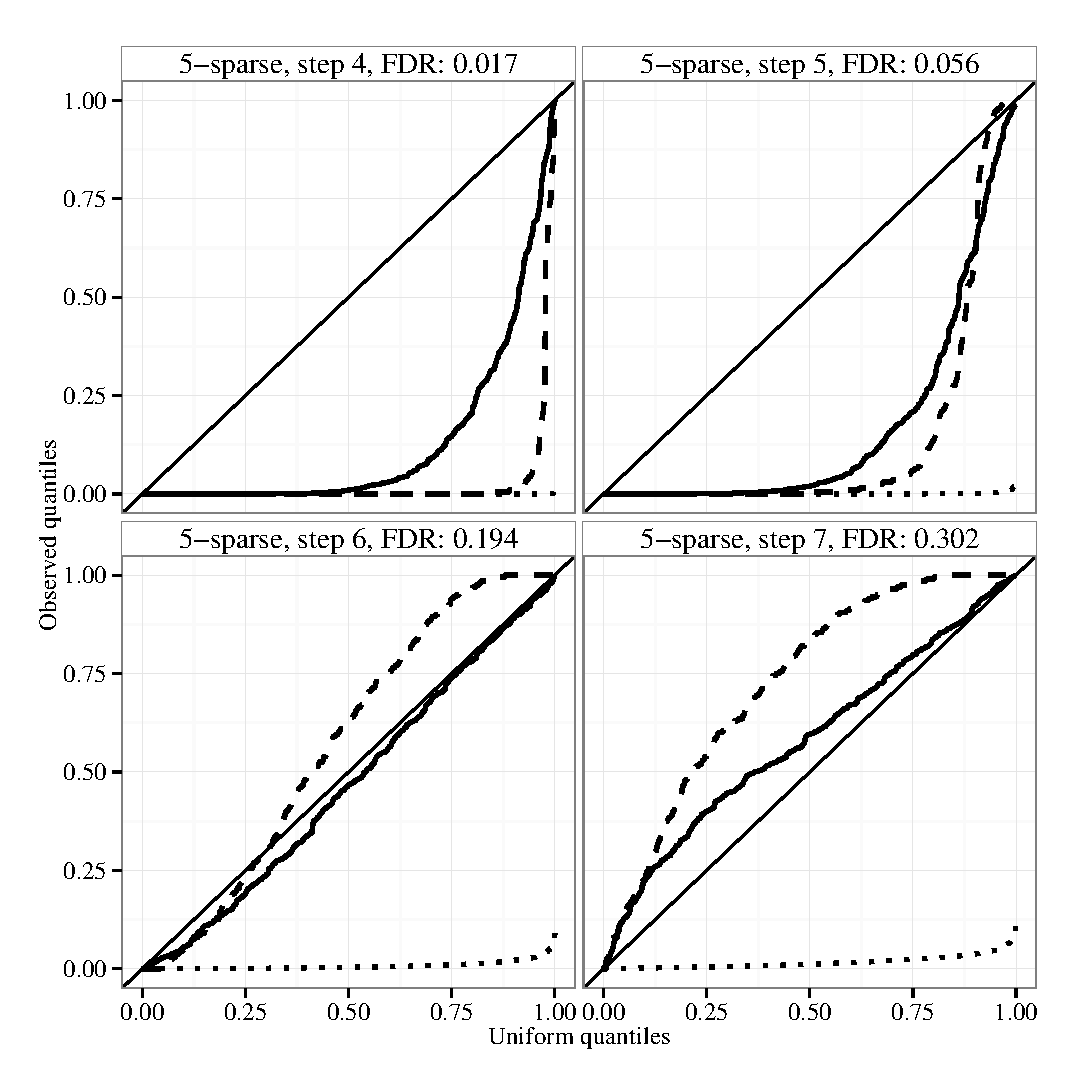
\includegraphics[width=.9\textwidth]{nonnull_G100_high4_binary.eps}
\caption{Quantile-quantile plots of test statistics computed at various steps in forward stepwise. Design matrices are random with $n = 100$ rows and $p = 200$ columns encoding $G = 100$ binary predictors generated from a Beta-Bernoulli model. Nonzero entries of $\beta$ are multiples of $\sqrt{2 \log (p)/n}$ with multipliers between 4 and 2. The outcome is $y_i = x_i\beta + \epsilon_i$ with $\epsilon_i \sim N(0,1)$. Lines are solid for $T\chi$, dashed for the Monte-Carlo estimate, and dotted for $\chi^2$.}
\label{fig:binary}
\end{center}
\end{figure}

\begin{figure}
\begin{center}
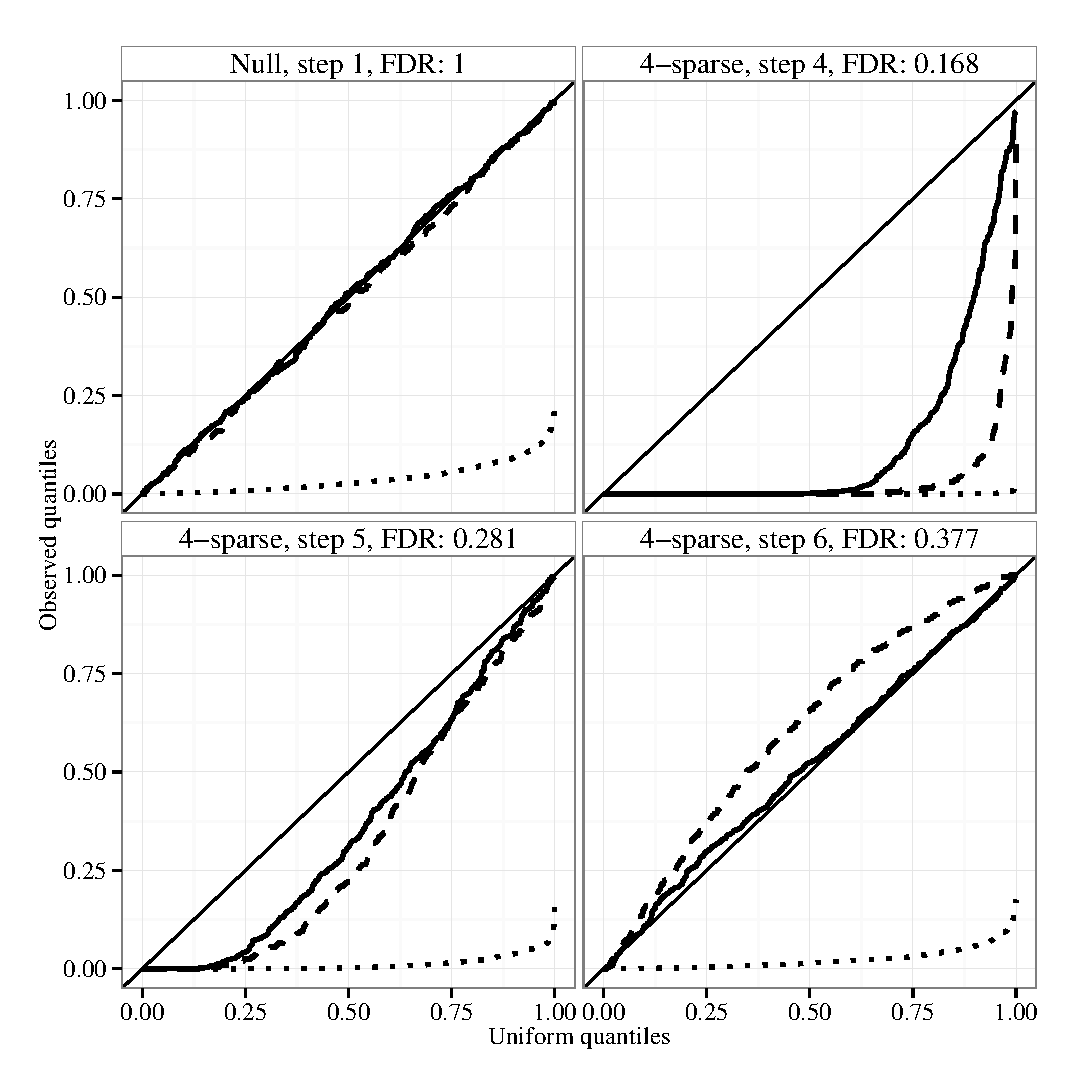
\includegraphics[width=.9\textwidth]{nonnull_G200_high15_data.eps}
\caption{Quantile-quantile plots of test statistics computed at various steps in forward stepwise. The design matrix has $n = 120$ rows and $p = 200$ columns consisting of gene expression data from microarray experiments. Nonzero entries of $\beta$ are multiples of $\sqrt{2 \log (p)/n}$ with multipliers between 15 and 12. The outcome is $y_i = x_i\beta + \epsilon_i$ with $\epsilon_i \sim N(0,1)$. Lines are solid for $T\chi$, dashed for the Monte-Carlo estimate, and dotted for $\chi^2$.}
\label{fig:eyedata}
\end{center}
\end{figure}

\begin{figure}
\begin{center}
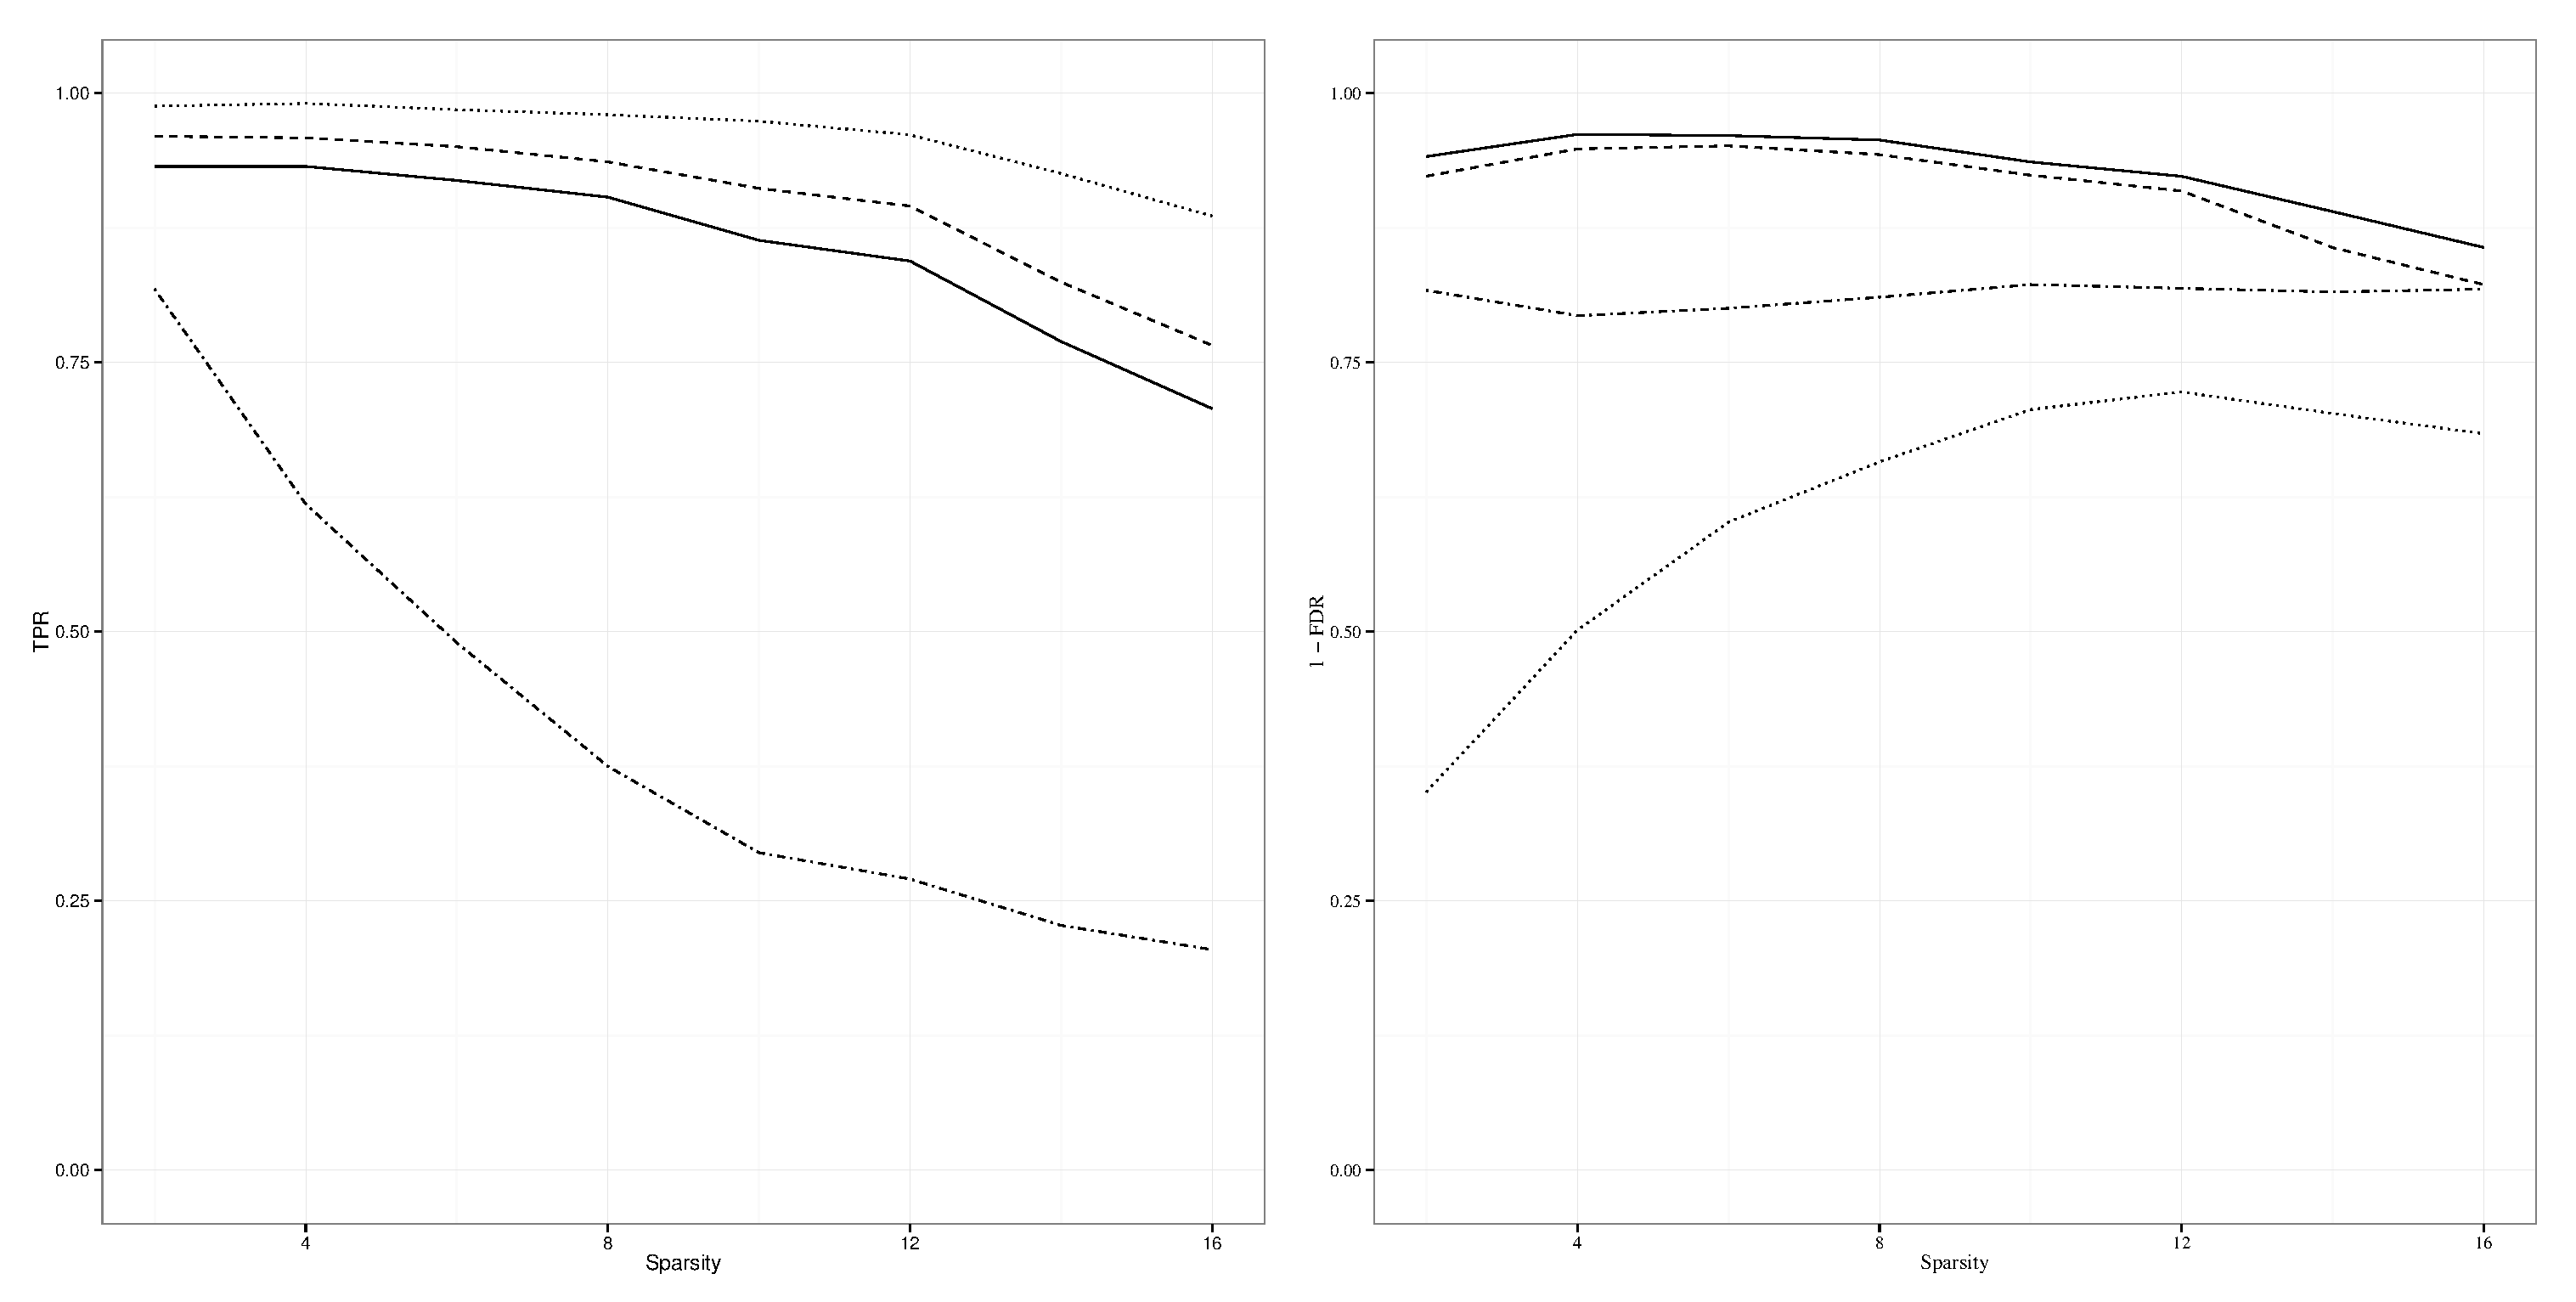
\includegraphics[width=\textwidth]{selection_G200_high2.eps}
\caption{\em For various sparsity levels $k$, the true positive rate
  in the left panel and 1 minus the false discovery rate in the right
  panel, for models selected by forward stepwise using various
  stopping criteria. Design matrices have standard Gaussian entries
  with $n = 100$ rows and $p = 200$ columns. Nonzero entries of
  $\beta$ are multiples of $\sqrt{2 \log (p)/n}$ with multipliers
  between 2 and 1.5. Forward stepwise ran with 50 steps and from the
  resulting sequence models were selected by \bic, dotted, by \ric,
  dashed, by \forward in \cite{sequential:fdr}, dot-dash, and by
  \last, described in equation \eqref{eq:klast}, solid.}
\label{fig:selection_sparsity}
\end{center}
\end{figure}

\begin{figure}
\begin{center}
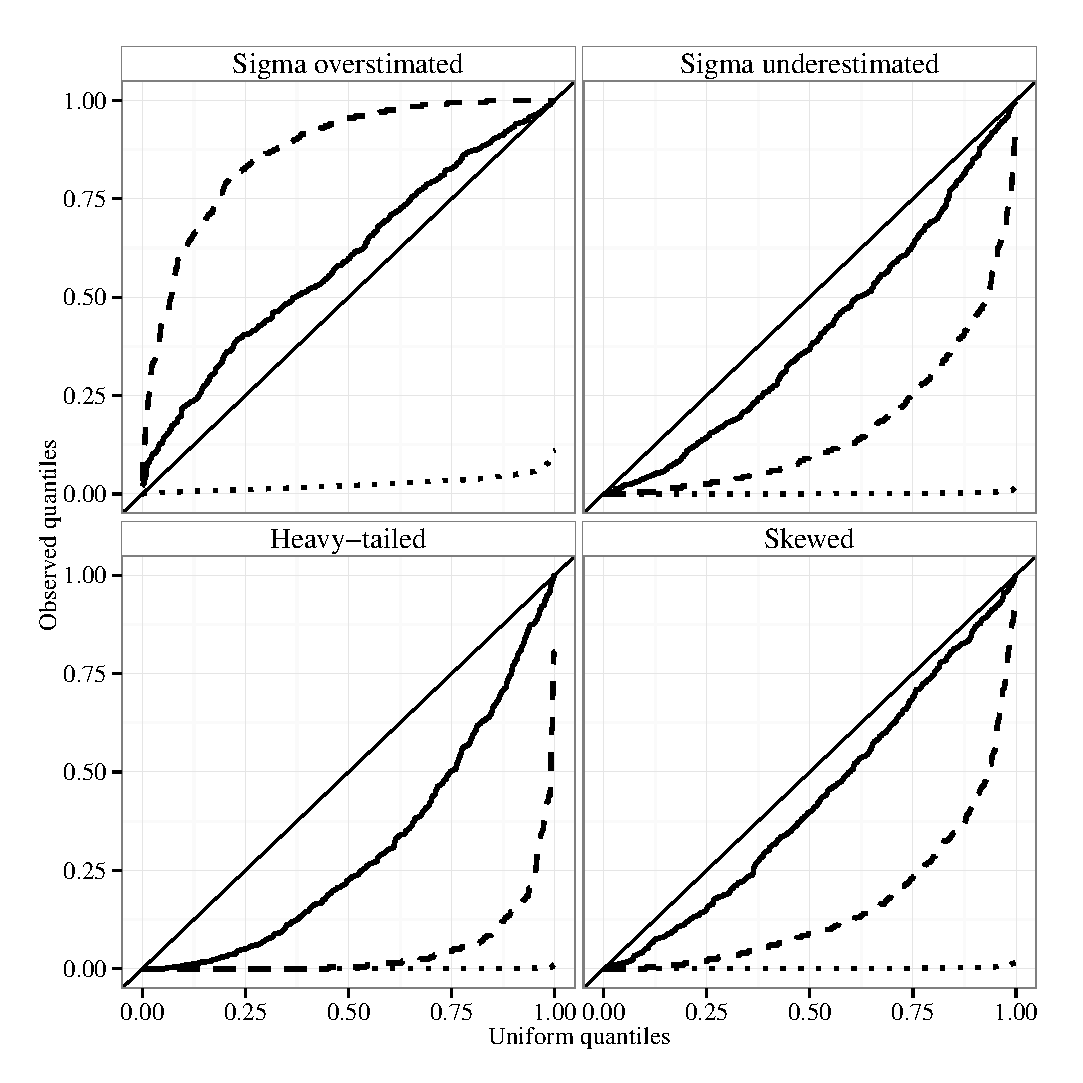
\includegraphics[width=.9\textwidth]{global_null_G200.eps}
\caption{Test statistic behavior when the noise distribution is not correctly specified. For overestimated and underestimated plots, the true $\sigma$ is 20\% smaller or larger, respectively, than the value used in computing each statistic. Heavy-tailed errors are from a $t$-distribution with standard error 50\% larger, using 18/5 degrees of freedom. Skewed errors are a standard normal plus a lognormal, with standard error 50\% larger than assumed. Lines are solid for $T\chi$, dashed for the Monte-Carlo test, and dotted for $\chi^2$. All plots are at the first step and under the global null.}
\label{fig:noisedist}
\end{center}
\end{figure}


\end{document}

